\section*{Аннотация}
\normalsize{    В работе необходимо исследовать явление вкустического резонанса
в тонком стержне; измерить скорость распространения продольных 
звуковых колебаний в тонких стержнях из различных материалов
и различных размеров; измерить модули Юнга различных материалов.}
\section*{Оборудование}
\begin{itemize}
    \item\normalsize{Частотомер}
    \item\normalsize{Осциллограф}
    \item\normalsize{Электромагнитные излучатель и приемник колебаний}
    \item\normalsize{Набор стержней из различных материалов}
\end{itemize}

\section*{Теоретические сведения и экспериментальная установка} \\[6pt]
\normalsize{    Скорость $u$ распространения продольной акустической волны в случае 
тонкого длинного стержня определяется как:}
\begin{equation}
    u = \sqrt{\frac{E}{\rho}} \text{,}
\end{equation}
где $\rho$ - плотнотсь среды, $E$ - модуль Юнга.\\
\normalsize{    В работе мы рассматриваем наиболее простой случай распространения звуковой
волны в твердом теле - в длинном тонком стержне. С точки зрения распространения
волн стержень считается тонким при условии $\lambda \gg R$, где $\lambda$ - длина
звуковой волны в стержне; $R$ - радиус стержня.
Акустическая волна, распространяясь в стержне конечной длины $L$, 
испытывает отражение от торцов и если при этом на длине стержня укладываестя 
целое число полуволн, то отраженные волны будут складываться в фазе с 
падающими, что пирведет к резкому усилению амплитудыих колебаний и возникновению
акустического резонанса в стержне.}
\normalsize{При частотах гармонического возбуждения, совпадающих
с собственными частотами колебаний стрежня, резко увеличивается 
амплитуда колебаний и в стержне образуется стоячая волна. Тогда 
для $n$-oй гармоники можно записать:}
\begin{equation}
    u = 2L\frac{f_n}{n}\\
\end{equation}
\normalsize{    Схема установки приведена ниже.\\Исследуемый
стержень 5 размещается на стойке 10. Возбуждение и приём колебаний в
стержне осуществляются электромагнитными преобразователями 4 и 6,
расположенными рядом с торцами стержня. Крепления 9, 11 электромагнитов
дают возможность регулировать их расположение повысоте, а
также перемещать вправо-влево по столу 12.
Электромагнит 4 служит для возбуждения упругих механических продольных
колебаний в стержне. На него с генератора звуковой частоты 1 подаётся 
сигнал синусоидальной формы: протекающий в катушке электромагнита ток создаёт
пропорциональное ему магнитное поле, вызывающее ериодическое воздействие заданной частоты на торец стержня (к торцам
стержней из немагнитных материалов прикреплены тонкие стальные
шайбы). Рядом с другим торцом стержня находится аналогичный электромагнитный датчик 6, который служит для преобразования механических
колебаний в электрические. Принцип работы электромагнитных датчиков
описан подробнее ниже.
Сигнал с выхода генератора поступает на частотомер 2 и на вход
канала X осциллографа 3. ЭДС, возбуждаемая в регистрирующем электромагните 6, пропорциональная амплитуде колебаний торца стержня, усиливается усилителем 7 и подаётся на вход канала Y осциллографа.
Изменяя частоту генератора и наблюдая за амплитудой сигнала с регистрирующего датчика, можно определить частоту акустического резонанса
в стержне.}
\begin{figure}[ht]
  \centering
  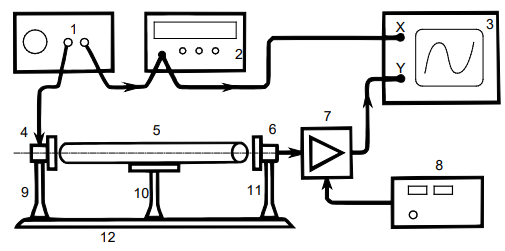
\includegraphics[width=8cm]{установка.png}
  \centering
  \caption{Схема установки: 1 – генератор звуковой частоты, 2 – частотомер,
3 – осциллограф, 4 – электромагнит-возбудитель, 5 – образец, 6 – электромагнитприёмник, 7 – усилитель звуковой частоты, 8 – блок питания усилителя,
9, 11 – стойки крепления электромагнитов, 10 – стойка крепления образца,
12 – направляющая}
\end{figure}
\section*{Экспериментальные данные}
\begin{table}[H]
    \centering
        \begin{tabular}{|c|c|c|c|c|}
            \hline
            \text{материал} & $d$ мм & $l$, мм & $m$, гр & $\rho$, кг/м^3 \\ \hline
            \text{медь} & 12.34 & 29.7 & 29.109 & 8195\\ \hline
            \text{дюралюминий} &  12.15 & 41.2 & 13.312 & 2786.79\\ \hline
            \text{сталь} &  12.38 & 41.2 & 37.084 & 7377.53\\ \hline
        \end{tabular}
        \caption{Плотность стрежней}
        \label{tab:my_labe_1}
\end{table}

\begin{table}[H]
        \centering
        \begin{tabular}{|c|c|c|c|c|c|}
            \hline
            $N$ & 1 & 2 & 3 & 4 & 5 \\ \hline
            $\nu_{\text{м}}$, кГц & 3.2182 & 6.4717 & 9.6619 & 12.884 & 16.106\\ \hline
            $\nu_{\text{a}}$, кГц & 4.2438 & 8.4857 & 12.6295 & 16.8745 & 21.21163\\ \hline
            $\nu_{\text{с}}$, кГц & 4.1278 & 8.2581 & 12.387 & 16.511 & 20.635\\ \hline
        \end{tabular}
        \caption{Резонансная частота стержней}
        \label{tab:my_labe_2}
\end{table}
\begin{figure}[H]
  \centering
  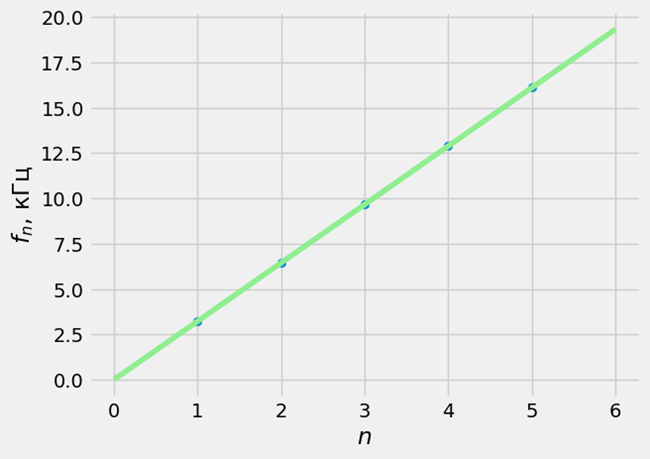
\includegraphics[width=8cm]{медь.png}
  \centering
  \caption{График зависимости резонансной частоты медного стержня от номера гармоники}
\end{figure}
\begin{figure}[H]
  \centering
  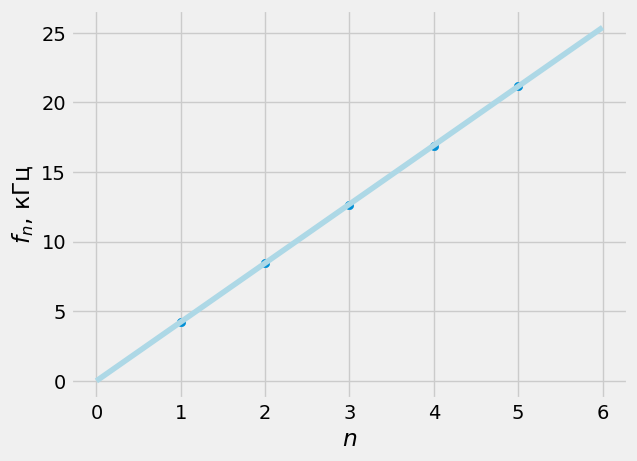
\includegraphics[width=8cm]{алюминий.png}
  \centering
  \caption{График зависимости резонансной частоты дюралюминиего стержня от номера гармоники}
\end{figure}
\begin{figure}[H]
  \centering
  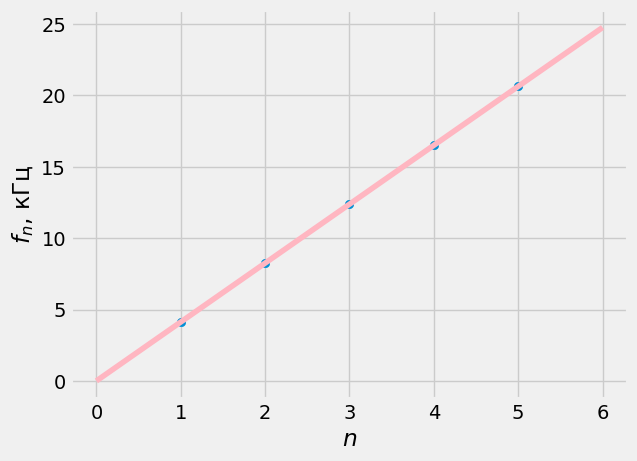
\includegraphics[width=8cm]{сталь.png}
  \centering
  \caption{График зависимости резонансной частоты стального стержня от номера гармоники}
\end{figure}
\begin{table}[H]
    \centering
    \begin{tabular}{|c|c|c|c|}
        \hline
        \text{величина/материал} & медь & дюралюминий & сталь\\ \hline
        $u$, м/с & 3862.79 & 5078.4 & 4952.4\\ \hline
        $E$, ГПа & 122.28 & 71.87 & 183.4\\ \hline
    \end{tabular}
    \caption{Резонансная частота стержней}
    \label{tab:my_labe_3}
\end{table}

\section*{Погрешности и результаты измерений}
\normalsize{    Погрешности вычисления плотности стержней определим по формуле:}
\begin{equation}
    \varepsilon_{\rho} = \sqrt{\left(\frac{\sigma_{m}}{m}\right)^2 + \left(\frac{\sigma_{l}}{l}\right)^2 + \left(\frac{\sigma_{d}}{d}\right)^2}
\end{equation}
\normalsize{    Погрешность вычисления скорости распределеня звуковых колебаний 
в стержнях определим по формуле:}
\begin{equation}
    \varepsilon_{u} = \sqrt{\left({\frac{\sigma_{k}}{k}\right)^2 + \left(\frac{\sigma_{l}}{L}\right)^2} \text{,}
\end{equation}
\normalsize{где k - наклон прямой графика зависимости $f_n(n)$, a $\sigma_k$:}
\begin{equation}
\sigma_k = \sqrt{\frac{\langle n^2\rangle \langle {f_n}^2\rangle - {\langle nf_n\rangle}^2}{n\langle n^2\rangle}}
\end{equation}
\normalsize{    Погрешность вычисления модуля Юнга определяется формулой:}
\begin{equation}
    \varepsilon_{E} = \sqrt{4{\varepsilon_{u}}^2 + {\varepsilon_{\rho}}^2} \approx \varepsilon_{\rho}
\end{equation}

\begin{table}[H]
    \centering
    \begin{tabular}{|c|c|c|c|}
        \hline
        \text{величина/материал} & медь & дюралюминий & сталь\\ \hline
        $\varepsilon_{\rho}$, $\%$  & 4.7  & 5.7 & 4.4\\ \hline
        $\varepsilon_{u}$, $\%$ & 0.1 & 0.17 & 0.08\\ \hline
        $\varepsilon_{E}$, $\%$ & 4.7 & 5.7 & 4.4\\ \hline
    \end{tabular}
    \caption{Погрешность измерений плотности, скорости и модуля Юнга стержней}
    \label{tab:faults}
\end{table}
\normalsize{Получаем:}
\begin{table}[H]
    \centering
    \begin{tabular}{|c|c|c|c|}
        \hline
        \text{величина/материал} & \text{медь} & \text{дюралюминий} & \text{сталь}\\ \hline
        $u \pm \sigma_{u}$, м/с & 3863 $\pm$ 4 & 5874 $\pm$ 9 & 4952 $\pm$ 4\\ \hline
        $E \pm \sigma_E$, ГПа & 122 $\pm$ 6 & 72 $\pm$ 4 & 183 $\pm$ 8\\ \hline
    \end{tabular}
    \caption{Результаты измерений}
\end{table}

\section*{Определение добротности колебательной системы}
\normalsize{Добротность $Q$ колебательной системы определяется как:}
\begin{equation}
    Q \sim \frac{\Delta f}{f_{\text{рез}}} \text{,}
\end{equation}
\normalsize{где $\Delta f$ - ширина резонанса}
\normalsize{$\Delta f = 0.0008$кГц, $f_{\text{рез}} = 3.2184$, тогда $Q \sim 2000$}\\
\section*{Выводы}
\nomalsize{В работе мы с помощью метода акустического резонанса измерили скорость распространения
продольных звуковых колебаний в тонких стержнях разных материалов, а так же измерили
модулю Юнга для них. Сравним результаты:}
\begin{table}[H]
    \centering
    \begin{tabular}{|c|c|c|c|}
        \hline
        \text{величина/материал} & \text{медь} & \text{дюралюминий} & \text{сталь}\\ \hline
        $u_{\text{эксп}} \pm \sigma_{u}$, м/с & 3863 $\pm$ 4 & 5874 $\pm$ 9 & 4952 $\pm$ 4\\ \hline
        $u_{\text{табл}}$, м/с & 3790 & - & 5150\\ \hline
        $E_{\text{эксп}} \pm \sigma_E$, ГПа & 122 $\pm$ 6 & 72 $\pm$ 4 & 183 $\pm$ 8\\ \hline
        $E_{\text{табл}}$, ГПа & 105-130 & 70.5 & 200-210 \\ \hline
    \end{tabular}
    \caption{Сравнение табличных данных с результатами эксперимента}
\end{table}
\normalsize{ Как можно видеть из $\ref{tab:faults}$ погрешность 
измерения модуля Юнга определяются погрешностью измерения 
плотности материала. Тогда сравним табличные и экспериментальные значения плотности:}
\begin{table}[H]
    \centering
    \begin{tabular}{|c|c|c|c|}
        \hline
        \text{величина/материал} & \text{медь} & \text{дюралюминий} & \text{сталь}\\ \hline
        $\rho_{\text{эксп}} \pm \sigma_{\rho}$, кг/$\text{м}^3$ & 8195 $\pm$ 386 & 2786 $\pm$ 159 & 7477 $\pm$ 331\\ \hline
        $\rho_{\text{табл}}$, кг/$\text{м}^3$  & - & 2800 & 7500-7900\\ \hline
    \end{tabular}
    \caption{Сравнение табличных данных с результатами эксперимента}
\end{table}
\normalsize{Плотность материалов входит в ворота погрешности.}
\normalsize{Погрешность скорости распространения продольных волн в стрежне мала, т.к относительная погрешность
как измерения частоты, так и измерения длины стержня много меньше единицы. Расхождения с табличными значениями
можно объяснить наличием иных примесей в сплавах стержней.}



